\chapter{Plasmonic Nanomaterials}\label{sec:background:Plasmonics}

\begin{itemize}
    \item Brief literature overview of nanostructure fabrication, brief history of plasmonic nanomaterials.
    \item Recent advances in the fabrication of nano-scale, tailor-designed structures have allowed the exploration of novel optical effects arising from the interaction between light and nanomaterials. Perhaps most commonly exploited are plasmonic materials: metallic structures within a dielectric environment whose optical properties are affected not only by material choice, but also their structural geometry.
    \item Find some seminal paper about plasmonic materials
\end{itemize}
The general response of a metal surface to incident light can be modelled in terms of plasma oscillations. By treating the metal as a free-electron gas (plasma) surrounding a lattice of positive charges, the electromagnetic response can be described by the motion of this plasma in response to external electromagnetic fields. 
At a metal-dielectric interface, incident light can drive electron-density waves that propagate along the metal surface. The coupled electromagnetic radiation and electron-density waves are known as surface plasmon polaritons (SPPs), and will propagate along the metal-dielectric interface, with an exponentially decaying intensity normal to the surface. 

\begin{figure}[htb!]
    \centering
    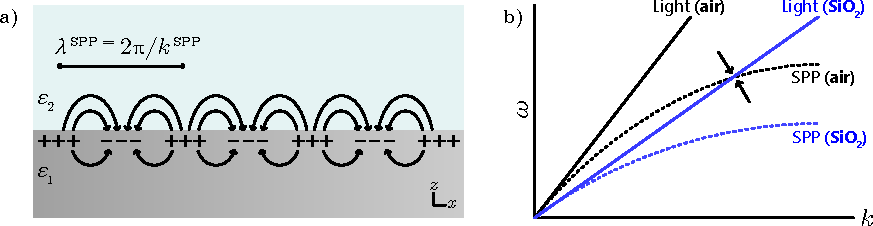
\includegraphics[scale=1.0]{./figures/background/plasmonics/spp.pdf}
    \caption{\label{fig:background:Plasmonics:SPP} \textbf{a)} Schematic of a surface plasmon polariton, of wavevector $k^{SPP}$, at a metal-dielectric interface. Charge density waves form in the metal surface, leading to surface-localised electromagnetic fields at the dielectric interface. \textbf{b)} Representative dispersion curves for surface plasmon polaritons and light at the interface of air or SiO$_2$. For any particular interface, SPPs cannot be excited by light impinging from the dielectric at that interface. Light propagating through glass can however be phase-matched to a SPP at a metal-air interface, for example. The momentum-matching point is illustrated with arrows. }
\end{figure}

We consider an interface between a metal and a dielectric, of permittivities $\varepsilon_1$ and $\varepsilon_2$ respectively (figure~\ref{fig:background:Plasmonics:SPP}a). The metal necessarily has permittivity ${\mathop{\rm Re}\nolimits}(\varepsilon_1)<0$. Excitation of SPPs require the real parts of $\varepsilon_1$ and $\varepsilon_2$ to be of opposite sign, that is, the interface is between a conductor and an insulator. In this configuration, the dispersion relation for a surface plasmon polariton propagating in the $x$ direction, oscillating at frequency $\omega$, is given by equation~\ref{eq:Plasmonics:SPPdispersion}~\cite[\S 2.2]{Maier2007}. 
\begin{equation}\label{eq:Plasmonics:SPPdispersion}
    k^{SPP}_{x} = k_0 \sqrt{\frac{\varepsilon_{1}\varepsilon_{2}}{\varepsilon_{1}+\varepsilon_{2}}} = \frac{\omega}{c} \sqrt{\frac{\varepsilon_{1}\varepsilon_{2}}{\varepsilon_{1}+\varepsilon_{2}}}
\end{equation}
For light incident on the interface via the dielectric described by $\varepsilon_2$, the optical dispersion relation $k_0 = \omega / c = \omega \sqrt{\mu_0 \varepsilon_2}$ shows that the optical momentum in the direction of SPP propagation will always be lower than that of the SPP (figure~\ref{fig:background:Plasmonics:SPP}b). Conservation of momentum must be considered when optically exciting surface plasmon polaritons, and so SPPs cannot be excited by light incident from the same dielectric as at the metal interface. Various experimental configurations have been demonstrated to allow the excitation of SPPs with optical radiation~\cite{Maier2007, Roh2011}, most commonly the Kretschmann and Otto geometries. These involve exciting a SPP at a metal-dielectric interface with light propagating through a different dielectric, interacting at an adjacent interface. In order for momentum matching to be properly realised, the projection of $k_0$ onto the axis of SPP propagation must match, and so depends strongly on the angle of optical incidence. Importantly for many applications, this angle is highly sensitive to changes in the dielectric environment. This allows the characterisation molecules attached to the metal surface by scanning the angle of incidence and observing induced shifts, leading to applications in molecular sensing and characterisation~\cite{Roh2011}.

In this work, we make use of plasmonic structure with characteristic dimensions comparable to, or smaller than, the wavelength of light in order to alleviate the momentum matching conditions. In these cases, the surface plasmons are confined to the nanoparticle surface, and are known as localised surface plasmons.


\section{Localised Surface Plasmons}\label{sec:background:Plasmonics:Metamaterials}

For small diameter $d \ll \lambda$ metallic nanoparticles, the phase of an oscillating electromagnetic field can be assumed constant over the particle, known as the ``quasi-static approximation''. In this approximation, the electron gas is driven to coherently oscillate at the particle surface. The lowest-order response of the particle to incident light can thus be described by an induced dipole moment $\bf{\tilde p}$, much like the simple Lorentz oscillator in section~\ref{sec:background:NonlinearOptics:lorentz} (figure~\ref{fig:background:Plasmonics:LSP}a).
For a metallic nanoparticle of permittivity $\varepsilon_1$ surrounded by a dielectric of permittivity $\varepsilon_2$, the induced dipole moment is described by equation~\ref{eq:Plasmonics:LSPdipole}. 
\begin{equation}\label{eq:Plasmonics:LSPdipole}
    {\bf{\tilde p}} = {\bf{\tilde \alpha }}{\bf{\tilde E}}
\end{equation}
As in section~\ref{sec:background:Chirality:opticalchirality}, $\bf{\tilde \alpha }$ describes the complex electric polarisability of the particle, and depends strongly on the nanoparticle material, geometry, and the permittivity of the surrounding medium.
Importantly, the induced dipolar plasmon mode is non-propagating, and so the momentum-matching requirements for exciting propagating surface plasmon polaritons are alleviated. The localised surface plasmon can be coherently excited by any oscillating electromagnetic field, and will reach a maximum excitation efficiency at a particular resonant frequency determined by the effective polarisability ${\tilde \alpha }(\omega)$ of the nanoparticle.
Analytical expressions for ${\tilde \alpha }(\omega)$ are well established for simple spherical nanoparticles of radius $a \ll \lambda$ and permittivity $\varepsilon(\omega)$~\cite{Maier2007, Collins2017}, given by equation~\ref{eq:Plasmonics:LSPalphaSphere}. 
\begin{equation}\label{eq:Plasmonics:LSPalphaSphere}
    {\tilde \alpha } = 4\pi a^3 \frac{\varepsilon (\omega) - \varepsilon_2 (\omega)}{\varepsilon (\omega) + 2\varepsilon_2 (\omega)}
\end{equation}
At the point where $\lvert \varepsilon (\omega) + 2\varepsilon_2 (\omega) \rvert$ is at it's minimum, i.e $\varepsilon (\omega) = -2\varepsilon_2 (\omega)$, the polarisability is maximally enhanced, determining the resonant frequency of the localised surface plasmon. However, in many systems the nanoparticle geometry is significantly more complex, and the LSP resonance cannot be determined analytically. Regardless of the particle geometry however, a particular resonant frequency will exist at which the plasmonic nanoparticle will resonantly scatter. Similar to surface plasmon polaritons, the sensitivity of the resonant frequency to the dielectric environment makes spectral analysis of the plasmonic scattering a sensitive technique for characterising nearby molecules, and has also gained popularity in molecular sensing applications~\cite{Petryayeva2011a, Polavarapu2014, Cheng2015}.

Another interesting application of deep sub-wavelength plasmonic nanostructures it the possibility of fabricating artificial ``metamaterials''. In arrays of nanoparticles supporting localised surface plasmons, the system can be modelled as an array of oscillators with effective polarisabilities. The macroscopic behaviour of the array can then be described as an effective medium, with a susceptibility describing its optical response as in section~\ref{sec:background:NonlinearOptics:susceptibility}. Now, the macroscopic optical properties of the metamaterial are strongly related to the geometry of the individual nanoparticle inclusions, offering unprecedented flexibility to design materials exhibiting optical properties never observed in nature. An often cited example of this is the possibility of a perfect optical lens formed from a metamaterial with negative refractive index, as proposed by Veselago~\cite{Veselago1968}, and later expanded on by Pendry~\cite{Pendry2000}. Further work has proposed the use of metamaterials for photonic devices such as perfect reflectors~\cite{Moitra2015}, polarisation optics~\cite{Cong2015}, and chiral-optical devices, expanded on in section~\ref{sec:background:Plasmonics:chiralPlasmonics}.


\begin{figure}[htb!]
    \centering
    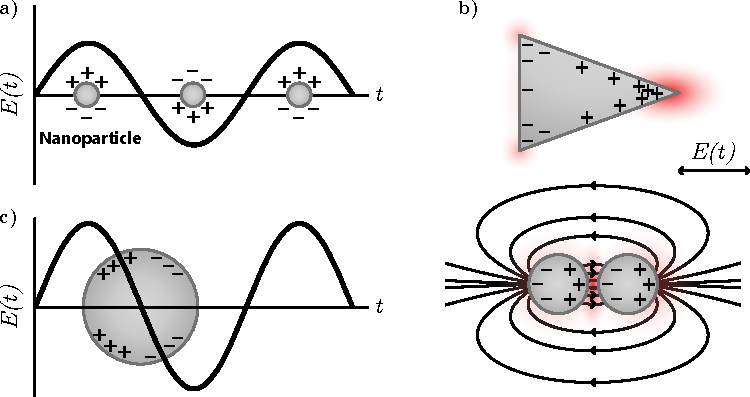
\includegraphics[scale=1.0]{./figures/background/plasmonics/lsp.pdf}
    \caption{\label{fig:background:Plasmonics:LSP} \textbf{a)} For sub-wavelength metallic nanoparticles, charge is coherently driven at the surface, and the particle can be approximated to an oscillating dipole. \textbf{b)} A pair of nanoparticles separated by some small distance will couple via the near-field, and function as a single dipole with an additional capacitance from the gap. Charge is efficiently confined to the inner surface, resulting in an enhanced electric field intensity between the two particles.}
\end{figure}



\subsection{Electromagnetic Field Confinement}\label{sec:Plasmonics:confinement}
\begin{itemize}
    \item Enhancement via localised surface plasmon resonance (excitation/scattering). 
    \begin{itemize}
        \item When a metallic nanoparticle is excited close to a plasmon resonance, the induced dipole oscillates at maximum amplitude. This results in a resonant scattering and absorption of light, leading to locally enhanced electromagnetic fields around the particle. 
        \item For sub-wavelength nanoparticles, this allows for sub-wavelength field confinement. The localised surface plasmon mode volume is limited by the particles sub-wavelength dimensions. Since the local electromagnetic field is determined by the, now tightly confined, surface plasmon mode, coupling this mode to incident light results in a confined local electromagnetic field at the particle surface.
        \item Example of enhancement from single nanoparticles
    \end{itemize}
    \item Enhancement via coupled localised surface plasmons (capacitance)
        \begin{itemize}
            \item A simple example is a pair of sub-wavelength nanoparticles, separated by a distance $d \ll \lambda$. This system behaves as a pair of point dipoles interacting via the near-field (figure~\ref{fig:background:Plasmonics:LSP}b). In the limit of small separation $d$, the coupled system will radiate as a dipole, and resonantly scatter when excited by light at it's resonant frequency. However, when driven by a field polarised along the chain axis, the gap between particles introduces a capacitance dependent on particle geometry and separation. This capacitance shifts the resonant frequency of the hybridised plasmon mode along that axis.
            \item Crucially, the capacitance of the gap results in the confinement of charge on the inner surfaces of the particles. This confinement of charge directly leads to confinement of the electromagnetic fields in the region between particles.
            \item Example of enhancement from coupled nanoparticles
        \end{itemize}
    \item Enhancement via lightning-rod effect (charge confinement)
    \begin{itemize}
        \item An additional enhancement in field confinement can come from the ``lightning-rod effect''. In the context of electrostatics, the lightning-rod effect describes the confinement of electric fields at sharp gradients of conducting structures, such as corners or tapered tips. Charge is confined more efficiently to regions of sharp surface gradients on a charged conductor, and so the electric field lines at the surface of the conductor will generally be localised around these sharp features.
        \item While not necessarily a relevant enhancement when considering coupled spherical nanoparticles, nanostructure geometries with sharper features, especially when multiple sharp features are closely coupled to each other, can greatly benefit from the additional confinement associated with the lightning-rod effect.
        \item Examples of field hotspots at the edges of nanostructures
        \begin{itemize}
            \item Direct observation of near-field localisation around the sharp features of a chiral nanostructure by ``nano-jets''~\cite{Valev2012d}
        \end{itemize}
    \end{itemize}
    
    \item Applications (literature review)
    \begin{itemize}
        \item Frequently used for SERS
        \item Sub-wavelength imaging (brief)
        \item Enhancement in chiral-optical measurements. Anything NOT about superchiral light, eg molecules between coupled spherical nanoparticles (see review sections).
        \item Enhanced nonlinear effects (due to strong intensity dependence) (most relevant to this work)
    \end{itemize}
\end{itemize}

\section{Beyond the Quasi-Static Approximation}
\begin{itemize}
    \item Intermediate regime of nanostructures, beyond the quasi-static approximation. Structure dimensions are close to, or larger than, the wavelength.
    \item The near-field optical behaviour in this regime can be understood in terms of higher order current density modes.
    \begin{itemize}
        \item The geometry of the metallic surface will permit a set of plasmon modes.
        \item Higher order plasmon modes can be excited across the surface of the structure.
        \item These modes are non-propagating standing waves, and have zero net momentum. Thus, even in this intermediate regime momentum matching is not a requirement to excite surface plasmons.
    \end{itemize}
    \item Literature review
    \begin{itemize}
        \item Zheng's work demonstrated that the plasmonic response of metallic nanostructures in this intermediate regime can be decomposed into a set of current density eigenmodes~\cite{Zheng2012}. This work was extended to collections of coupled nanostructures~\cite{Zheng2013}. 
        \item The optical response can be further understood by applying group theory to the plasmonic eigenmode set~\cite{Zheng2015}, allowing the current density modes to be grouped by the optical polarisation states that exclusively excite them.
    \end{itemize}
\end{itemize}


\section{Chiral Plasmonic Nanostructures} \label{sec:background:Plasmonics:chiralPlasmonics}
\begin{itemize}
    \item Freedom of fabrication techniques allow symmetries to be explored.
    \item Second-order nonlinear processes, which already enhance chiroptical measurements, can themselves be enhanced as described in section~\ref{sec:Plasmonics:confinement}.
    \item Literature review. Lots of references in~\cite[\S 3.2]{Collins2017}
\end{itemize}

\subsection{Superchiral Fields from Plasmonic Metasurfaces}
\begin{itemize}
    \item Literature review (directly from \cite[\S 4.3]{Collins2017})
\end{itemize}